%% bare_conf.tex
%% V1.3
%% 2007/01/11
%% by Michael Shell
%% See:
%% http://www.michaelshell.org/
%% for current contact information.
%%
%% This is a skeleton file demonstrating the use of IEEEtran.cls
%% (requires IEEEtran.cls version 1.7 or later) with an IEEE conference paper.
%%
%% Support sites:
%% http://www.michaelshell.org/tex/ieeetran/
%% http://www.ctan.org/tex-archive/macros/latex/contrib/IEEEtran/
%% and
%% http://www.ieee.org/

%%*************************************************************************
%% Legal Notice:
%% This code is offered as-is without any warranty either expressed or
%% implied; without even the implied warranty of MERCHANTABILITY or
%% FITNESS FOR A PARTICULAR PURPOSE!
%% User assumes all risk.
%% In no event shall IEEE or any contributor to this code be liable for
%% any damages or losses, including, but not limited to, incidental,
%% consequential, or any other damages, resulting from the use or misuse
%% of any information contained here.
%%
%% All comments are the opinions of their respective authors and are not
%% necessarily endorsed by the IEEE.
%%
%% This work is distributed under the LaTeX Project Public License (LPPL)
%% ( http://www.latex-project.org/ ) version 1.3, and may be freely used,
%% distributed and modified. A copy of the LPPL, version 1.3, is included
%% in the base LaTeX documentation of all distributions of LaTeX released
%% 2003/12/01 or later.
%% Retain all contribution notices and credits.
%% ** Modified files should be clearly indicated as such, including  **
%% ** renaming them and changing author support contact information. **
%%
%% File list of work: IEEEtran.cls, IEEEtran_HOWTO.pdf, bare_adv.tex,
%%                    bare_conf.tex, bare_jrnl.tex, bare_jrnl_compsoc.tex
%%*************************************************************************

% *** Authors should verify (and, if needed, correct) their LaTeX system  ***
% *** with the testflow diagnostic prior to trusting their LaTeX platform ***
% *** with production work. IEEE's font choices can trigger bugs that do  ***
% *** not appear when using other class files.                            ***
% The testflow support page is at:
% http://www.michaelshell.org/tex/testflow/



% Note that the a4paper option is mainly intended so that authors in
% countries using A4 can easily print to A4 and see how their papers will
% look in print - the typesetting of the document will not typically be
% affected with changes in paper size (but the bottom and side margins will).
% Use the testflow package mentioned above to verify correct handling of
% both paper sizes by the user's LaTeX system.
%
% Also note that the "draftcls" or "draftclsnofoot", not "draft", option
% should be used if it is desired that the figures are to be displayed in
% draft mode.
%
\documentclass[conference]{IEEEtran}
% Add the compsoc option for Computer Society conferences.
%
% If IEEEtran.cls has not been installed into the LaTeX system files,
% manually specify the path to it like:
% \documentclass[conference]{../sty/IEEEtran}

% Some very useful LaTeX packages include:
% (uncomment the ones you want to load)

% *** MISC UTILITY PACKAGES ***
%
%\usepackage{ifpdf}
% Heiko Oberdiek's ifpdf.sty is very useful if you need conditional
% compilation based on whether the output is pdf or dvi.
% usage:
% \ifpdf
%   % pdf code
% \else
%   % dvi code
% \fi
% The latest version of ifpdf.sty can be obtained from:
% http://www.ctan.org/tex-archive/macros/latex/contrib/oberdiek/
% Also, note that IEEEtran.cls V1.7 and later provides a builtin
% \ifCLASSINFOpdf conditional that works the same way.
% When switching from latex to pdflatex and vice-versa, the compiler may
% have to be run twice to clear warning/error messages.

% *** CITATION PACKAGES ***
%
%\usepackage{cite}
% cite.sty was written by Donald Arseneau
% V1.6 and later of IEEEtran pre-defines the format of the cite.sty package
% \cite{} output to follow that of IEEE. Loading the cite package will
% result in citation numbers being automatically sorted and properly
% "compressed/ranged". e.g., [1], [9], [2], [7], [5], [6] without using
% cite.sty will become [1], [2], [5]--[7], [9] using cite.sty. cite.sty's
% \cite will automatically add leading space, if needed. Use cite.sty's
% noadjust option (cite.sty V3.8 and later) if you want to turn this off.
% cite.sty is already installed on most LaTeX systems. Be sure and use
% version 4.0 (2003-05-27) and later if using hyperref.sty. cite.sty does
% not currently provide for hyperlinked citations.
% The latest version can be obtained at:
% http://www.ctan.org/tex-archive/macros/latex/contrib/cite/
% The documentation is contained in the cite.sty file itself.






% *** GRAPHICS RELATED PACKAGES ***
%
\ifCLASSINFOpdf
  % \usepackage[pdftex]{graphicx}
  % declare the path(s) where your graphic files are
  % \graphicspath{{../pdf/}{../jpeg/}}
  % and their extensions so you won't have to specify these with
  % every instance of \includegraphics
  % \DeclareGraphicsExtensions{.pdf,.jpeg,.png}
\else
  % or other class option (dvipsone, dvipdf, if not using dvips). graphicx
  % will default to the driver specified in the system graphics.cfg if no
  % driver is specified.
  % \usepackage[dvips]{graphicx}
  % declare the path(s) where your graphic files are
  % \graphicspath{{../eps/}}
  % and their extensions so you won't have to specify these with
  % every instance of \includegraphics
  % \DeclareGraphicsExtensions{.eps}
\fi
% graphicx was written by David Carlisle and Sebastian Rahtz. It is
% required if you want graphics, photos, etc. graphicx.sty is already
% installed on most LaTeX systems. The latest version and documentation can
% be obtained at:
% http://www.ctan.org/tex-archive/macros/latex/required/graphics/
% Another good source of documentation is "Using Imported Graphics in
% LaTeX2e" by Keith Reckdahl which can be found as epslatex.ps or
% epslatex.pdf at: http://www.ctan.org/tex-archive/info/
%
% latex, and pdflatex in dvi mode, support graphics in encapsulated
% postscript (.eps) format. pdflatex in pdf mode supports graphics
% in .pdf, .jpeg, .png and .mps (metapost) formats. Users should ensure
% that all non-photo figures use a vector format (.eps, .pdf, .mps) and
% not a bitmapped formats (.jpeg, .png). IEEE frowns on bitmapped formats
% which can result in "jaggedy"/blurry rendering of lines and letters as
% well as large increases in file sizes.
%
% You can find documentation about the pdfTeX application at:
% http://www.tug.org/applications/pdftex





% *** MATH PACKAGES ***
%
%\usepackage[cmex10]{amsmath}
% A popular package from the American Mathematical Society that provides
% many useful and powerful commands for dealing with mathematics. If using
% it, be sure to load this package with the cmex10 option to ensure that
% only type 1 fonts will utilized at all point sizes. Without this option,
% it is possible that some math symbols, particularly those within
% footnotes, will be rendered in bitmap form which will result in a
% document that can not be IEEE Xplore compliant!
%
% Also, note that the amsmath package sets \interdisplaylinepenalty to 10000
% thus preventing page breaks from occurring within multiline equations. Use:
%\interdisplaylinepenalty=2500
% after loading amsmath to restore such page breaks as IEEEtran.cls normally
% does. amsmath.sty is already installed on most LaTeX systems. The latest
% version and documentation can be obtained at:
% http://www.ctan.org/tex-archive/macros/latex/required/amslatex/math/





% *** SPECIALIZED LIST PACKAGES ***
%
%\usepackage{algorithmic}
% algorithmic.sty was written by Peter Williams and Rogerio Brito.
% This package provides an algorithmic environment fo describing algorithms.
% You can use the algorithmic environment in-text or within a figure
% environment to provide for a floating algorithm. Do NOT use the algorithm
% floating environment provided by algorithm.sty (by the same authors) or
% algorithm2e.sty (by Christophe Fiorio) as IEEE does not use dedicated
% algorithm float types and packages that provide these will not provide
% correct IEEE style captions. The latest version and documentation of
% algorithmic.sty can be obtained at:
% http://www.ctan.org/tex-archive/macros/latex/contrib/algorithms/
% There is also a support site at:
% http://algorithms.berlios.de/index.html
% Also of interest may be the (relatively newer and more customizable)
% algorithmicx.sty package by Szasz Janos:
% http://www.ctan.org/tex-archive/macros/latex/contrib/algorithmicx/




% *** ALIGNMENT PACKAGES ***
%
%\usepackage{array}
% Frank Mittelbach's and David Carlisle's array.sty patches and improves
% the standard LaTeX2e array and tabular environments to provide better
% appearance and additional user controls. As the default LaTeX2e table
% generation code is lacking to the point of almost being broken with
% respect to the quality of the end results, all users are strongly
% advised to use an enhanced (at the very least that provided by array.sty)
% set of table tools. array.sty is already installed on most systems. The
% latest version and documentation can be obtained at:
% http://www.ctan.org/tex-archive/macros/latex/required/tools/


%\usepackage{mdwmath}
%\usepackage{mdwtab}
% Also highly recommended is Mark Wooding's extremely powerful MDW tools,
% especially mdwmath.sty and mdwtab.sty which are used to format equations
% and tables, respectively. The MDWtools set is already installed on most
% LaTeX systems. The lastest version and documentation is available at:
% http://www.ctan.org/tex-archive/macros/latex/contrib/mdwtools/


% IEEEtran contains the IEEEeqnarray family of commands that can be used to
% generate multiline equations as well as matrices, tables, etc., of high
% quality.


%\usepackage{eqparbox}
% Also of notable interest is Scott Pakin's eqparbox package for creating
% (automatically sized) equal width boxes - aka "natural width parboxes".
% Available at:
% http://www.ctan.org/tex-archive/macros/latex/contrib/eqparbox/





% *** SUBFIGURE PACKAGES ***
%\usepackage[tight,footnotesize]{subfigure}
% subfigure.sty was written by Steven Douglas Cochran. This package makes it
% easy to put subfigures in your figures. e.g., "Figure 1a and 1b". For IEEE
% work, it is a good idea to load it with the tight package option to reduce
% the amount of white space around the subfigures. subfigure.sty is already
% installed on most LaTeX systems. The latest version and documentation can
% be obtained at:
% http://www.ctan.org/tex-archive/obsolete/macros/latex/contrib/subfigure/
% subfigure.sty has been superceeded by subfig.sty.



%\usepackage[caption=false]{caption}
%\usepackage[font=footnotesize]{subfig}
% subfig.sty, also written by Steven Douglas Cochran, is the modern
% replacement for subfigure.sty. However, subfig.sty requires and
% automatically loads Axel Sommerfeldt's caption.sty which will override
% IEEEtran.cls handling of captions and this will result in nonIEEE style
% figure/table captions. To prevent this problem, be sure and preload
% caption.sty with its "caption=false" package option. This is will preserve
% IEEEtran.cls handing of captions. Version 1.3 (2005/06/28) and later
% (recommended due to many improvements over 1.2) of subfig.sty supports
% the caption=false option directly:
%\usepackage[caption=false,font=footnotesize]{subfig}
%
% The latest version and documentation can be obtained at:
% http://www.ctan.org/tex-archive/macros/latex/contrib/subfig/
% The latest version and documentation of caption.sty can be obtained at:
% http://www.ctan.org/tex-archive/macros/latex/contrib/caption/




% *** FLOAT PACKAGES ***
%
%\usepackage{fixltx2e}
% fixltx2e, the successor to the earlier fix2col.sty, was written by
% Frank Mittelbach and David Carlisle. This package corrects a few problems
% in the LaTeX2e kernel, the most notable of which is that in current
% LaTeX2e releases, the ordering of single and double column floats is not
% guaranteed to be preserved. Thus, an unpatched LaTeX2e can allow a
% single column figure to be placed prior to an earlier double column
% figure. The latest version and documentation can be found at:
% http://www.ctan.org/tex-archive/macros/latex/base/



%\usepackage{stfloats}
% stfloats.sty was written by Sigitas Tolusis. This package gives LaTeX2e
% the ability to do double column floats at the bottom of the page as well
% as the top. (e.g., "\begin{figure*}[!b]" is not normally possible in
% LaTeX2e). It also provides a command:
%\fnbelowfloat
% to enable the placement of footnotes below bottom floats (the standard
% LaTeX2e kernel puts them above bottom floats). This is an invasive package
% which rewrites many portions of the LaTeX2e float routines. It may not work
% with other packages that modify the LaTeX2e float routines. The latest
% version and documentation can be obtained at:
% http://www.ctan.org/tex-archive/macros/latex/contrib/sttools/
% Documentation is contained in the stfloats.sty comments as well as in the
% presfull.pdf file. Do not use the stfloats baselinefloat ability as IEEE
% does not allow \baselineskip to stretch. Authors submitting work to the
% IEEE should note that IEEE rarely uses double column equations and
% that authors should try to avoid such use. Do not be tempted to use the
% cuted.sty or midfloat.sty packages (also by Sigitas Tolusis) as IEEE does
% not format its papers in such ways.





% *** PDF, URL AND HYPERLINK PACKAGES ***
%
%\usepackage{url}
% url.sty was written by Donald Arseneau. It provides better support for
% handling and breaking URLs. url.sty is already installed on most LaTeX
% systems. The latest version can be obtained at:
% http://www.ctan.org/tex-archive/macros/latex/contrib/misc/
% Read the url.sty source comments for usage information. Basically,
% \url{my_url_here}.





% *** Do not adjust lengths that control margins, column widths, etc. ***
% *** Do not use packages that alter fonts (such as pslatex).         ***
% There should be no need to do such things with IEEEtran.cls V1.6 and later.
% (Unless specifically asked to do so by the journal or conference you plan
% to submit to, of course. )


% correct bad hyphenation here
\hyphenation{op-tical net-works semi-conduc-tor}

\usepackage[colorlinks]{hyperref}
%\usepackage[inner=2cm,outer=2cm,bottom=2cm,top=3cm]{geometry}
\usepackage{wrapfig}
\usepackage{subfigure}
\usepackage{xspace}
%%%%%%%%%%%%%%%%%%%%%%%%%%%%%%%%%%%%%%%%%
% Acronym of the proposal
\newcommand{\proposal}{DISCUTE\xspace}
%%%%%%%%%%%%%%%%%%%%%%%%%%%%%%%%%%%%%%%%%
%% TODO macros
\usepackage[textwidth=17mm]{todonotes}
  \newcommand{\customtodo}[4]{
        \todo[color=#2,inline,size=\small]{
                \ifx&#3&
                        \textbf{#1} #4
                \else
                        \textbf{#1$\Rightarrow$#3} #4
                \fi
        }
  }
\usepackage{ifthen}
\newboolean{WIP}
\gdef\ifwip{\ifthenelse{\boolean{WIP}}}
%\setboolean{WIP}{false}%
\setboolean{WIP}{true}%
\ifwip{
  \newcommand{\AL}[2][]{\customtodo{AL}{green!50}{#1}{#2}}
  \newcommand{\MS}[2][]{\customtodo{MS}{red!20}{#1}{#2}}
  \newcommand{\JP}[2][]{\customtodo{JP}{blue!20}{#1}{#2}}
  \newcommand{\FQ}[2][]{\customtodo{FQ}{brown!20}{#1}{#2}}
}{ % else if WIP = false
  \newcommand{\AL}[2][]{}
  \newcommand{\MS}[2][]{}
  \newcommand{\JP}[2][]{}
  \newcommand{\FQ}[2][]{}
}
%% End of todo macros
%%%%%%%%%%%%%%%%%%%%%%%%%%%%%%%%%%%%%%%%%
%% Italic abreviations, ...
\newcommand{\ie}[0]{{\em i.e.},\xspace}
\newcommand{\vs}[0]{{\em vs.}\xspace}
\newcommand{\eg}[0]{{\em e.g.},\xspace}
\newcommand{\etal}[0]{{\em et al.}\xspace}
\newcommand{\wrt}[0]{{\em w.r.t.}\xspace}
\newcommand{\aka}[0]{{\em a.k.a.}\xspace}
%%%%%%%%%%%%%%%%%%%%%%%%%%%%%%%%%%%%%%%%%

\newcommand{\sg}{SimGrid\xspace}
\newcommand{\vmps}{VMps\xspace}
\begin{document}
%
% paper title
% can use linebreaks \\ within to get better formatting as desired
\title{\vmps -- A Generic Tool to Investigate and Compare VM Placement Algorithms}


% author names and affiliations
% use a multiple column layout for up to three different
% affiliations
\author{\IEEEauthorblockN{Adrien Lebre, Jonathan Pastor, Mario S\"{u}dholt}
\IEEEauthorblockA{ASCOLA Research Group (Mines Nantes, Inria, Lina), France\\ firstname.lastname@inria.fr
}}



% make the title area
\maketitle

\thispagestyle{plain}
\pagestyle{plain}

\begin{abstract}
%\boldmath
The abstract goes here.
\end{abstract}
% IEEEtran.cls defaults to using nonbold math in the Abstract.
% This preserves the distinction between vectors and scalars. However,
% if the conference you are submitting to favors bold math in the abstract,
% then you can use LaTeX's standard command \boldmath at the very start
% of the abstract to achieve this. Many IEEE journals/conferences frown on
% math in the abstract anyway.

% no keywords




% For peer review papers, you can put extra information on the cover
% page as needed:
% \ifCLASSOPTIONpeerreview
% \begin{center} \bfseries EDICS Category: 3-BBND \end{center}
% \fi
%
% For peerreview papers, this IEEEtran command inserts a page break and
% creates the second title. It will be ignored for other modes.
\IEEEpeerreviewmaketitle



\section{Introduction}
\label{sec:intro}
%\AL[AL]{1 page (including the abstract)}

Although a lot of progress has been made on Cloud Computing (CC)
system managements, \aka Infrastructure-as-a-Service
toolkits~\cite{moreno:2012}, most of them are still leveraging
elementary Virtual Machine (VM) placement policies that prevent them
% AL -> MS, blabla and blibli -> blabla WHILE bliblibli, I want to
% highlight that both objectives should be addressed simultaneously
from maximizing the usage of CC resources while guaranteeing VM
resources requirements, \aka Service Level Agreements (SLAs).
%% THE TEXT BELOW COMES FROM ISPA'13
%%%%%%%
Typically, a batch scheduling approach is used: VMs are (i)~allocated
according to user requests for resource reservations, and (ii)~tied to
the nodes where they were deployed until their destruction. Besides
the fact that user requests are often overestimated, such policies are
definitely not optimal for CC providers, since the effective resource
requirements of each operated VM may significantly vary during its
execution.
%%%%%%%
It is rather surprising that most available IaaS
toolkits~\cite{openstack, opennebula, cloudstack} continue to rely on
greedy, static allocation approaches as more flexible and often more
efficient approaches to the Virtual Machine Placement Problem (VMPP)
have been developed by the research community. Dynamic strategies such
as consolidation, load balancing and other SLA-ensuring algorithms
have been deeply investigated
\cite{Hermenier:2009:ECM:1508293.1508300}, \cite{feller:ccgrid12},
\cite{quesnel:cpe2012}, \cite{5935254}, \cite{5715067},
\cite{5328077}.  From our point of view, an important impediment to
the adoption of such advanced strategies is related to the
experimental process that has been used to validate the pros and cons
of each of them: most VMPP proposals have been evaluated either by
leveraging ad-hoc simulators or small testbeds. These evaluation
environments are not accurate and not representative enough to (i)
ensure their correctness on real platforms and (ii) perform fair
comparisons between them.

%
\begin{figure}[ht]
\vspace*{-.2cm}
\begin{center}
        \subcapcentertrue
        \subfigure[Scheduling steps]{
        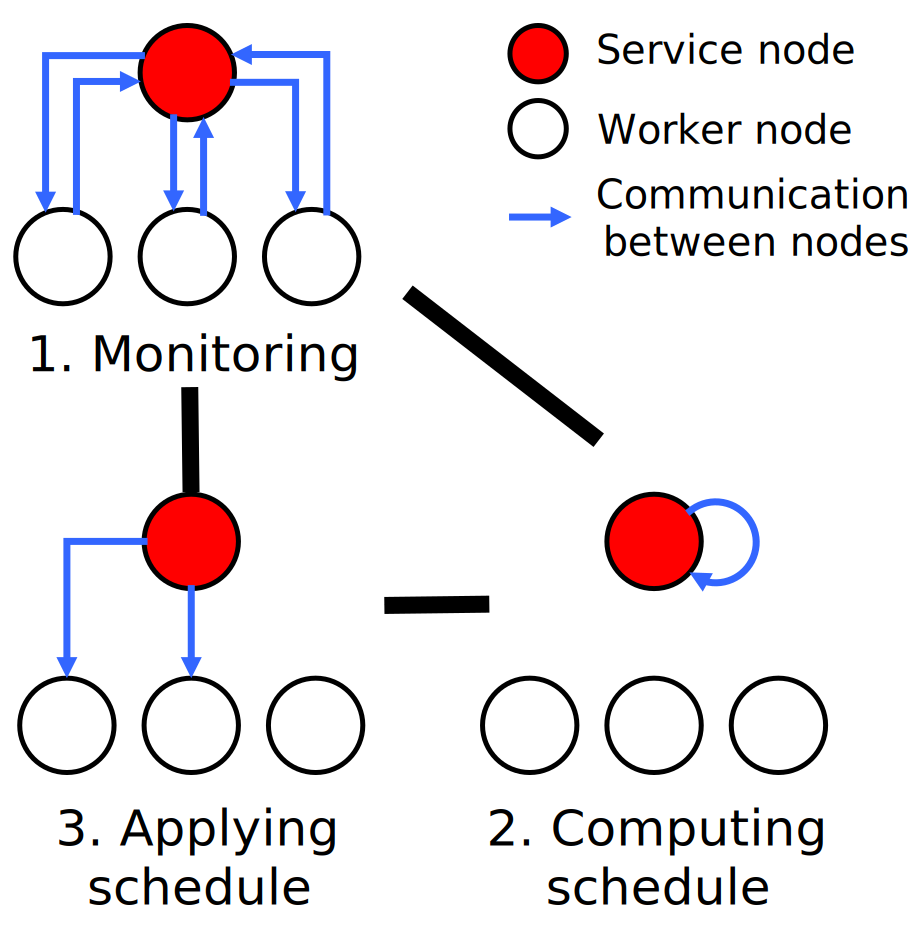
\includegraphics[width=.45\linewidth]{figures/scheduling_steps.pdf}
        \label{fig:scheduling_steps}}
        \subfigure[Workload fluctuations during scheduling]{
        \includegraphics[width=.45\linewidth]{figures/workload_fluctuations2.pdf}
        \label{fig:workload_fluctuations}}
\vspace*{-.2cm}
\caption{VM scheduling in a master/worker architecture}
\end{center}
\label{fig:scheduling}
\vspace*{-.2cm}
\end{figure}
%
Each VMPP mechanism is a complex system that can face
important side-effects during each of its stages: Monitoring the
resources usages, computing the schedule and applying the
reconfiguration (see Figure \ref{fig:scheduling_steps}).
%
%
As an example, a single master architecture can lead, \textit{a priori} to
important drawbacks. First, during the computation and the application
of a schedule, a single master cannot take into account new VM
requirement violations. Second, the time needed to apply a new
schedule can be particularly important: The longer the reconfiguration
process, the higher the risk that the schedule may be outdated, due to
the workload fluctuations, when it is eventually applied (see Figure
\ref{fig:workload_fluctuations}). Finally, a single master node can
lead to well-known fault-tolerance issues: A group of VMs may be
temporarily isolated from the master node in case of a network
disconnection or if the master node crashes.
%
Implementing each proposal and evaluating it on representative
testbeds in terms of scalability, reliability and workload changes
would definitely be the most rigorous way to observe and propose
appropriate solutions to aforementioned
side-effects.
% and compare  with existing proposals.
However, \textit{in-vivo} (\ie real-world) experiments, if it is
possible to execute them, are always expensive and tedious to perform;
they may even be counterproductive if their results lead to false
conclusions, \eg because of errors due to involving unanticipated
interferences of different parts of the experiments that cannot be
explored sufficiently in complex real-world environments.

In this article, we propose % the first version of
\vmps, a dedicated simulation framework to perform in-depth
investigations of VM placement algorithms and compare them with each
other in a fair way. To cope with real conditions such as the
increasing scale of modern data centers and the dynamicity of the
workloads that are specific to the Cloud Computing paradigm, notably
its elasticity capacity, \vmps allows users to study large-scale
scenarios that taking into account server crashes and that involve
tens of thousands of VMs, each one executing a specific workload that
evolves during the simulation lifetime.

We believe that such a tool will be beneficial to a large number of
researchers in the field of CC as it enables them to quickly validate
% AL->MS the characterisctics -> the trends,  simulations are
% well-known scientific intrusments to validate trends (and only trends).
the trends of a new proposal and compare it with existing
ones. This way, our approach allows \textit{in vivo} experiments to be
restricted to VMPP mechanisms that have the potential to handle CC
production infrastructures.

%
We chose to build \vmps on top of the \sg
toolkit~\cite{casanova:hal-01017319} since (i) its relevance in terms
of performance and validity has already been
demonstrated~\cite{simgridpub} and (ii) because it has been recently
extended to integrate virtual machine abstractions and a live
migration model \cite{Hirofuchi:2013:ALM:2568486.2568524}.

To illustrate the relevance of \vmps, we implemented the essential
mechanisms of three well-known VMPP approaches:
Entropy~\cite{Hermenier:2009:ECM:1508293.1508300},
Snooze~\cite{feller:ccgrid12}, and DVMS~\cite{quesnel:cpe2012}. We
have investigated their characteristics by analyzing their
scalability, reliability and reactivity (\ie the time to solve an SLA
violation). Besides being well-known from the literature, we chose
these three systems as they are built on three different software
architecture models: Entropy uses a centralized model, Snooze a
hierarchical one and DVMS a fully distributed one.

The experiments reveal ...
\AL[AL]{What the experiments reveal at the end ? }

The rest of the article is organized as follow. Section~\ref{sec:sg}
gives an overview of the \sg framework.  \ref{sec:injector} introduces
\vmps and discusses its general functioning.  The three algorithms
implemented as use-cases are presented in
Section~\ref{sec:vm-schedulers} and evaluated in
Section~\ref{sec:experiments}.  Section~\ref{sec:related} and
Section~\ref{sec:conclusion} present, respectively, related work as
well as a conclusion and future work.

\section{Simgrid, a generic toolkit}
\label{sec:sg}
%\AL[AL]{0.5page}

\sg is a simulation toolkit to study the behavior of
large-scale distributed systems.  Developped for more than  a decade, It has been used in more than 100
publications.  Its main characterisitics are related to its:
\begin{itemize}
\item Extensibility -- After Grids, HPC and P2P
  systems, \sg has been recently extended with virtualization technologies abstractions
(\ie Virtual Machines including a live migration model \cite{Hirofuchi:2013:ALM:2568486.2568524}) to allow users to investigate Cloud
Computing challenges \cite{lucas:cloud2014};
\item Scalability -- It is possible to simulate large-scale scenarios,
  as an example, users can simulate applications composed of 2
  Millions of processors and an infrastructure composed of 10,000~servers hosting more than
  100,000~VMs on a computer with 16~GB of memory;
\item  Flexibility -- It allows to run a simulation on arbitrary network
  topology under dynamic computation and network resources
  availabilities;
\item API --  users can leverage \sg through easy-to-use APIs in C
  and Java.
\end{itemize}

To perform simulations, users should develop a \emph{program} and
define a \emph{platform} file and a \emph{deployment} file. The
\emph{program} in most cases leverages the \sg MSG API that allow
end-users to create and execute \sg abstractions such as processes,
tasks, VMs and network-communications. The \emph{platform} file gives
the physical description of each resource composing the environment
and on which aforementioned computations/network exchanges will be
performed in the \sg
world.% (host, CPU capacity, network topology and link capacities, etc.)
Finally, the \emph{deployment} file is used to launch the different
\sg processes defined in the \emph{program} on the different nodes (at
lease the mapping between one process and one host is mandatory to
start the simulation). The execution of the program is orchestrated by
the \sg engine that internally relies on an constraint solver to
correctly assign the amount of CPU/network resources to each \sg
abstraction, step by step until the simulation ends.

Although SimGrid has many features such as model checking, the
simulation of DAGs (Direct Acyclic Graphs) or MPI applications, we
only give a brief description of the  virtualization  abstractions
that have been recently implemented in \sg and on which our framework relies
on.  Further information regarding \sg is available in \cite{casanova:hal-01017319}.

The VM support has been designed so that all operations that can be performed
o a host can be performed inside a VM: From the point of view of a \sg
Host, a \sg VM is considered as an ordinary task while from the point
of view of a task running inside a \sg VM, a VM is considered as an
ordinary host below the task.  By such a mean, \sg users can easily
switch between a virtualized and non virtualized infrastructure.
Moreover, thanks to  MSG API extensions, users can control VMs in the
same manner as in the real world (\eg create/destroy, start/shutdown,
suspend/resume and migrate).
% live migration
For migration operations, a VM live migration model implementing the
precopy migration algorithm of Qemu/KVM has been integrated into \sg.
This model is the only one that successfully simulates the live
migration behavior by taking into account the resource sharing
competition as well as the memory refreshing rate of the VM, thus
determining correctly the live migration time as well as the resulting
network traffic~\cite{Hirofuchi:2013:ALM:2568486.2568524}.

Those two capabilities were mandatory to build our VM placement
simulator toolkit introduced in the next section.

\section{VM Placement Simulator}
\label{sec:injector}
\AL[AL]{1.5 page}

The purpose of \vmps is to deliver a generic tool
to evaluate new VM placement algorithms and offer the possibility to
compare them each other. Concretely, it consists of a piece of code in
charge of managing VM creations, workload fluctuation changes as well
as node apparitions/removals so that researchers can focus on the
implementation of the new placement algorithm and evaluate how it
behaves according to the different changes that occur during the
simulation.
%
\vmps has been implemented in JAVA by
leveraging the corresponding MSG API of \sg.  Although the JAVA layer
has an impact of the efficiency of \sg, we believe it is rather
acceptable in comparison to the benefit that brings JAVA  to researchers to
implement advanced scheduling strategies.
\AL[JP]{Should we talk about SCALA ?}

After giving an overview of the framework, we describe  its general
functioning.% and how researchers can develop new algorithms

\subsection{Overview}
\label{sec:overview}

At coarse-grained, \vmps proceeds a simulation in three
phrases: (i) Initialization (ii) injection and (iii) traces analysis.
The initialization phase corresponds to the creation of the
environment, the VMs and the generation of the events queue. The
injection phase corresponds to the step where the scheduling strategy
is evaluated. Basically, it consists of at least two \sg processes,
one for the \emph{injector} and one for the scheduling algorithm.
Regarding the \emph{injector}, this is the generic part of the
framework. As it name suggest, it is in charge of injecting the
different events that occur during the execution of the simulations.
Current events are VM CPU load changes and node apparitions/removals.
% As we describe in the next section, additional events can be easily added.
\AL[AL]{Make two figures: a architectural one (i.e. Injector vs
  schedulers pool and one chronological.}

Regarding the scheduling algorithm, users should develop their own
algorithm by leveraging the java MSG API and the \texttt{XHost},
\texttt{XVM} and \texttt{SimulatorManager} classes. The two former
classes extend respectively the \sg \texttt{Host} and \texttt{VM}
abstractions while the latter aims at controlling the interactions
between the different components of the VM placement simulator.
Throughout these three classes, users can get at any time, the current
state of the infrastructure (\ie. the load of a  host/VM,
the number of VMs hosted on the whole infrastructure or on a particular
host, check whether one host is overloaded, etc.) To illustrate the
development of schedulers, \vmps is currently released with
three scheduling mechanisms described in Section
\ref{sec:vm-schedulers}. We choose this three mechanisms as they
investigate three different software architecture models: centralized,
hierarchical and distributed. Although we do not discuss that point
due to space constraints, we emphasize that delivering those three
mechanisms enables us to deliver concrete examples of
how the deployment file of \sg is automically generated by leveraging a
generic python script.
\AL{We should highlight that point in the README.org}
%DONE : \AL{We should explain the deployment file in the \sg section}
The last phase consists in analyzing the collected traces in order to
generate the different figures.

%\begin{itemize}
%\item Entropy \cite{Hermenier:2009:ECM:1508293.1508300}, a centralized approach using a constraint programming approach to solve the placement/reconfiguration VM problem;
% \item Snooze \cite{feller:ccgrid12}, a hierarchical approach where
%   each manager of a group invokes Entropy to solve the
%  placement/reconfiguration VM problem. It is noteworthy that in
%   \cite{feller:ccgrid12}, Snooze is using a specific heuristic to solve the placement/reconfiguration VM problem. As the sake of simplicity, we have simply reused the entropy scheduling code.
%\item  DVMS \cite{quesnel:cpe2012}, a distributed approach that dynamically partitions the system and invokes Entropy on each partition.
% \end{itemize}

\subsection{Initialization Phase}
At the beginning, \vmps creates $n$ VMs and assigns them in a
round-robin manner on the $p$ first hosts defined in the platform file.
The default platform file corresponds to a cluster of $p+s$ hosts,
where $p$ corresponds to the number of hosting nodes and $s$ to the
number of services nodes. The values $n$, $p$ and $s$ are given as input
parameters of each simulation (specified in a java properties file).
\AL[AL]{Update the size of the cluster autonomically by leveraging p +
s}
 Although the cluster topology is usually the
most common, it is possible to define more complex platforms to simulate for
instance, multi data centers scenarios.
%Note that $s$ can be equals to 0 if the
%scheduling strategy is directly executed on the hosting nodes .

Each VM is created based on one of the predefined VM classes. A VM
class corresponds to a template defining the VM attributes and its
memory footprint. Concretely, it is described as
\texttt{nb\_cpu:ramsize:net\_bw:mig\_speed:mem\_speed} where
\texttt{nb\_cpus} defines the number of cores, \texttt{ramsize} the
size of the memory, \texttt{net\_bw} the network bandwidth,
\texttt{mig\_speed} the maximum bandwidth available to perform the
migration and \texttt{mem\_speed} the maximum memory update speed when
the VM is consuming 100\% of its CPU resources. This last parameter
enables users to simulate different kinds of workload (\ie
memory-intensive vs non-intensive), which is mandatory to be inline
with real Cloud Computing conditions. We remind that the memory update
speed is a critical parameter that governs the migration time as well
as the amount of transferred data. Available classes are defined in a
specific text file that can be modified according to the user's needs.
For each VM creation, a process selects one class (\ie one line) in
the file randomly. Hence, if a user want to favor one class with
respect to another one, it is as simple as repeating the line of the
class more times. Finally, all VMs start with a CPU consumption of 0
that will evolve during the simulation as explained below.
We emphasize that each random process used in \vmps is initialized with a seed
that is defined in a configuration file. By such a mean, we can ensure
the reproducibility between the different simulations and thus fair
comparisons.

Once the creation and the assignment of VMs is completed, \vmps spawns at least two SG processes, the \emph{injector} and the
launcher of the selected scheduler.
The first action of the \emph{injector} consists in creating the
different events queues and merge them as a global one  that will be consumed during the second phase of the
simulation.  For the moment two kinds of events are generated: ~\emph{
 CPU load}
and \emph{node crash} events.
%The former consists in changing the load of a VM by
%creating  and assigning a new \sg task in the VM while the second aims
%at simulating crashes.
%
%Changing the load of a VM has a direct impact of its memory update speed and thus on the time
%to migrate it between two hosts.
Regarding the \emph{CPU load} events queue, it is generated in order to change every $t$
seconds in average the load of each VM. $t$ is a random variable that
follows an exponential distribution with rate parameter $\lambda\_t$
while the
CPU load of a VM evolves according to a Gaussian distribution defined by
a particular mean ($\mu$) as well as a particular standard deviation
($\sigma$). $t$, $\mu$ and $\sigma$ are given as input parameters of each
simulation.
As a CPU can fluctuate between 0 and 100\%, \vmps
prevents to assign non-sense values  when the Gaussian distribution returns a
number smaller than 0 or greater than 100. Although this has no impact
of the execution of the simulation, we highlight that this can  reduce/increase the
effective mean of the VM load, especially when $\sigma$ is high.
Hence, it is important for users to specify appropriate values.
\AL[AL]{A binomial law would have solved this issue: too late too bad :(}
%Although this can have an impact on the
%effective mean, especially when $\sigma$ is high, we believe it was
%non appropriated to request it is easier for end-users to specify $\mu$ and
%$\sigma$ parameters than

Regarding the \emph{node crash} events queue, it is generated in order to
turn off a node every $f$ seconds in average and for a duration of $d$ seconds.
Similarly to the previous $t$ value, $f$ follows an exponential
distribution with rate $\lambda\_f$. $f$ and $d$ are given as input
parameters of each simulation.

Adding new events can be easily done by simply defining new event
java classes implementing the \texttt{InjectorEvent} interface and by
adding the code in charge of generating the associated queue. Such a
new queue will be merged to the global one and its events will be
consume similarly to other ones during the
\emph{Injector Phase}.
\AL[AL]{Future work: introduce network changes}

\subsection{Injector Phase}
Once the VMs and the global event queue are ready, the evaluation of the
scheduling mechanism can start. On the first side, the injector
process will iteratively
consumes the different events. That is for the moment, changing the load of a VM or
turning off/on a node.
Changing the load of a VM corresponds to the
creation and the assignment of a new \sg task in the VM. This new task has
a direct impact since it increases or decreases the current memory
update speed of the VM and thus the time that is mandatory to migrate
it. \AL{Is it clear enough? }
% that is indicated by the \texttt{mem\_speed}
%% parameter given in the class description.
When a node is turning off, the VMs that were running on that node are
temporarily discarded, \ie they are hidden and cannot be access untill
the node comes back. By such a mean, the scheduler cannot considered
them.
\AL[AL, MS, JP]{This is ugly but unfortunately the true, it will be
  better to reassign those VMs on other nodes, but which one? }
As highlighted in Future work, we are investigating other
approaches that can better match real scenario usages such as turning
off the VMs and reprovisioning each one  on other nodes.
%
\AL{Future work: add the possibility to have VMs
  appearing/disappearing on the fly like a dynamic provisioning
  strategy}

According to the scheduling algorithm, VMs will be suspended/resumed or
relocated through the
different hosts to ensure scheduling objectives and SLA guarantees.
We highlight that users must implement the algorithm in charge of
solving the VMPP but also the code in charge of
applying the reconfiguration plan by invoking the appropriate methods
available through the \texttt{SimulatorManager} class. This step is
essential as the reconfiguration cost is a key element of dynamic
placement systems.
\AL{maybe it is better to prevent the access to Xhost and XVM methods
  that can change the Simulator States. Hence, we should enforce the
  access only through the SimulatorManager class ? What do you think ?}
Last but not the least, It is noteworthy that \vmps really invokes the execution of
each scheduling strategy in order to get the effective reconfiguration
plan.  That is, the computation time that is observed
is not simulated but corresponds to the effective one, only the
workload inside the VMs and the migration operations are simulated in
\sg. It is hence mandatory to propragate such a time into the \sg
engine by invoking a \texttt{wait} MSG call.

\subsection{Traces Analysis}
\label{subsec:traces-analysis}
The last step of \vmps consists in analysing the
information that has been collected during the simulation.
% in order to understand and compare the behavior of the different
% algorithms.
This analysis is done in a two-step fashion. First, \vmps records
several metrics related to the platform utilization throughout the
simulation by leveraging an extended version of the \sg TRACE
module~\footnote{http://simgrid.gforge.inria.fr/simgrid/3.12/doc/tracing.html}.
While keeping the possibility of using visualization tool
promoted by the \sg community such as PajeNG \cite{pageng:www},
this extension enables the creation of a trace file in the
JSON file format, which is  used, in a second time, to generate several figures
using the R program \cite{R:Bloomfield:2014}.

By default, \vmps records, the load of the different VMs/hosts, the
appearance and the duration of each VM requirements violation in the
system, the number of migration, the number of times the scheduler
mechanism has been invoked and the number of times it succeeds or
fails to resolve the non viable configurations.
%
Although such information are key elements to understand and
compare the behavior of the different algorithms, we highlight that
the TRACE API enables the creation of as many variable as necessary,
allowing researchers to instrument their own algorithm with specific
variables.

\section{Dynamic VM Placement Algorithms}
\label{sec:vm-schedulers}
To illustrate the interest of \vmps, we implemented three dynamic VM
placement mechanisms respectively based on the Entropy
\cite{Hermenier:2009:ECM:1508293.1508300}, Snooze
\cite{feller:ccgrid12}, and DVMS \cite{quesnel:cpe2012} proposals. For the three
implementations, we chose to use the latest VMPP solver that has been
developed as part of the Entropy
framework~\cite{Hermenier:2009:ECM:1508293.1508300, hermenier:cp11}.

%
Giving up consolidation
optimality in favor of scalability, this algorithm provides a ``repair
mode'' that enables the correction of VM requirement violations (\aka
SLA violations). The algorithm considers that a host is
overloaded when the VMs try to consume more than 100\% of the CPU
capacity of the host. In such a case, the algorithm looks for
an optimal viable configuration until it reaches a predefined timeout.
The optimal solution is a new placement that satisfies
the requirements of all VMs while minimizing the cost of the
reconfiguration.
Once the timeout has been triggered, the algorithm returns
the best solution among the ones it finds and applies the associated
reconfiguration plan by invoking live migrations in the simulation
world.

%
Although using the Entropy VMPP solver
implies a modification from the original Snooze proposal,  we
highlight that our goal is to illustrate the capabilities of \vmps and
thus we believe that such a modification is acceptable as it does not
change the global behavior of Snooze. Moreover by
conducting such a comparison, we also investigate the pros and cons of
the three  architecture models on which these proposals rely on (\ie centralized, hierarchical and
distributed).

%
Before discussing the simulation results, we
describe in this section an overview of the three implemented systems.

\subsection{Entropy-based Centralized Approach}
\label{subsec:entropy}
The centralized VM placement mechanism consists in one single \sg
process deployed on a service node. It implements a simple loop that
iteratively checks the viability of the current configuration by
invoking every $p$ seconds the aforementioned VMPP solver. $p$ is
defined as an input parameter of the simulation. As mentioned in
Section \ref{subsec:traces-analysis}, for each iteration, we monitor
whether the VMPP solver suceeded or failed. In case of success, \vmps
records the number of migration that has been performed and whether
the application of the reconfiguration plan led to new violations.
\AL{Should we explain the issue right now or not ? } Indeed, during
the computation and the application of a schedule, the algorithm does
not enforce QoS properties anymore, and thus cannot react quickly to
violations. Second, since the manipulation of VMs is costly, the time
needed to apply a new schedule is particularly important: The longer
the reconfiguration process, the higher the risk that the schedule may
be outdated, due to the workload fluctuations, when it is eventually
applied.
\vmps enables researchers to investigate such concerns in-depth.


% Pas de titre de section : il se trouve dans le fichier
\subsection{Snooze-based Hierarchical Approach}
\label{subsec:snooze}
We now present Snooze~\cite{feller:ccgrid12} as a second case study of how
to implement and simulate advanced algorithms.
We present its architecture summarizing its main
characteristics from its original presentation~\cite{feller:ccgrid12} and
additional information  stemming from personal communications of the Snooze
developers and its implementation~\cite{snoozeweb,snoozedev14}.

\subsubsection{Architecture}
\label{sec:snoozeArchi}

Snooze harnesses a hierarchical architecture in order to support load
balancing and fault tolerance, cf.\ Fig.~\ref{fig:snoozearch}.

\begin{figure}[hbp]
  \begin{center}
  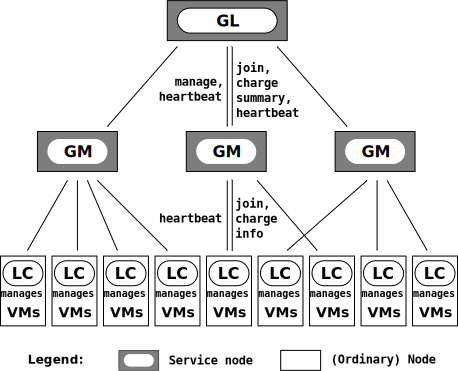
\includegraphics[width=.85\linewidth]{figures/snoozearch.pdf}
  \caption{Overview of Snooze's architecture}
  \label{fig:snoozearch}
\end{center}
\vspace*{-.3cm}
\end{figure}

At the
top of the hierarchy, a \emph{group leader (GL)} centralizes
information about the whole cluster using summary data about
\emph{group managers (GMs)} that constitute the intermediate layer of
the hierarchy. GMs manage a number of \emph{local controllers (LCs)}
that, in turn, manage the VMs assigned to nodes. The GL and the GMs
are deployed on service nodes while the LCs are executed on hosting
node.  During execution, higher-level components periodically send
heartbeats to lower-level ones; monitoring information, \eg about the
system load, is also sent periodically in the opposite direction. In
order to propagate information down the hierarchy, Snooze relies on
hardware support for multicast communication. Finally, a number of
replicated entry points allows clients to contact the GL, \eg in order
to submit new VMs for integration into the system.

\emph{Simulation using \vmps.~} The \texttt{XHOST}, \texttt{XVM} and
\texttt{SimulatorManager} classes have been harnessed to implement the
core architectural abstractions (\ie VM monitoring and manipulations),
the remaining concepts and algorithms of Snooze have been implemented
using Simgrid's primitives and standard Java mechanisms.
%
Communication between Snooze actors is implemented based on Simgrid's
primitives for, mainly asynchronous, event handling.
Hardware\-sup\-ported multicast communication that is used, \eg
to relay heartbeats, is implemented as a dedicated actor that manages
a state representing GL and GM heartbeat groups and relaying heartbeat
events.
%
Finally, our Snooze simulation uses, as its original counterpart, a
multi-threaded implementation (\ie based on multiple SG processes) in
order to optimize reactivity even for large groups of LCs (or GMs)
that have to be managed by one GM (or GL).

\subsubsection{Algorithms}
\label{sec:snoozeAlgs}

Apart from the handling of faults (described below), two types of
algorithms are of major importance for the administration of the
Snooze architecture: the algorithms that enable components to
dynamically enter the system and the algorithms that propagate info
between the components.

A GL is created, if it does not exist, by promotion of a GM that is
selected according to some leader election algorithm. When a GM joins
a cluster, it starts listening on a predefined channel for the
heartbeat of the GL and registers once it has received the
heartbeat. New LCs first also wait for the GL heartbeat, contact the
GL then in order to obtain a GM assignment, and finally register at
the GM assigned to them.

Two kinds of (load) information are passed within the system: the
periodic heartbeat message sent by the GL and the GMs; second,
periodic load information sent from LCs to their respective GMs and
summary load info sent by the GMs to the GL.

\subsubsection{Fault tolerance}

GLs, GMs and LCs may fail during the system execution. System
components identify that a node on the corresponding higher-level node
has failed (the GL in case of a GM, a GM in the case of an LC) in an
asynchronous fashion through the lack of heartbeat messages.

In the case of a GL failure, one of the GMs becomes the new GL, stops
its GM activities and prevents the LCs it manages so that they can
start rejoining the system. If a GM fails, the GL and the LCs it has
managed will become aware of it based on the lack of heartbeats,
update its data structures and, for the LCs, rejoin the system. If an
LC fails, its GM will finally learn of it due to the missing heartbeat
and charge information of the LC. The GM will then remove the LC from
its data structures.


% \subsubsection{Variants}
% \label{sec:snoozeVariants}

% Our simulation framework facilitates the simulation of variants of
% placement algorithms. In the following, we present three non-trivial
% variants that we have implemented and explored: a variant of the
% assignment algorithm of LCs to GMs, periodic vs.\ reactive scheduling,
% and a variant of the algorithms of how GMs and LCs join the system.


% \paragraph{Assignment of LCs to GMs}

% LCs are assigned to GMs by the GL as part of the LC join protocol. In
% Snooze's native implementation LCs are assigned in a round-robin
% fashion to the known GMs. If GMs join (and leave) the system at the
% same time as LCs, a round-robin strategy at join time, however, does
% not ensure an even distribution. This may happen, for instance at
% startup time of the system, when new GMs and LCs enter the system, or
% in case of failures, which trigger GM and LC joins. In order to
% evaluate the imbalance resulting from a round-robin strategy (as well
% as others) we have implemented the LC assignment protocol in a modular
% fashion and applied it in diverse highly-dynamic settings in which GMs
% and LCs enter the system at the same time. Furthermore, we have
% implemented a best-fit strategy that assigns LCs to GMs with minimal
% load or to GMs with the smallest number of assigned LCs (if several
% GMs with minimal load exist). The best-fit strategy can significantly
% improve the scheduling characteristics of hierarchical placement
% algorithms as shown by the experimental data presented in
% Sec.~\ref{sec:snoozeVariantsEval}. Furthermore, it should always be
% at least as good as the round-robin strategy (the corresponding proof
% is left to future work).


% \paragraph{Periodic vs.\ reactive scheduling}

% Snooze~\cite{feller:ccgrid12} schedules VMs in a periodic fashion:
% after a fixed time period a GM calls the scheduler in order to resolve
% resource conflicts among the LCs it manages. The information whether a
% resource conflict has to be handled is taken based on the summary
% information that is periodically sent by the LCs to the GM.

% We have provided an alternative, reactive, strategy to scheduling: as
% soon as they occur, LCs avert their GMs of resource conflicts; the GMs
% then initiate scheduling. Implementing this reactive scheme can be
% done using our framework in two manners: either by implementing
% additional asynchronous transmissions as a real implementation of the
% necessary state updates would proceed or, in a much more lightweight
% manner, through direct accesses by the GMs to the states of their
% respective LCs. While the latter does not mimic a real implementation
% closely, it can be harnessed to yield a valid simulation: delays
% induced by communication in the ``real'' implementation, for instance,
% can be easily added as part of the lightweight simulation. We have
% implemented this lightweight variant of reactive scheduling.


% \paragraph{Variants of the join algorithms}

% The join algorithms, see Sec.~\ref{sec:snoozeAlgs}, are crucial to the
% correctness of Snooze for two main reasons: (i) they have to be
% efficient because they can easily form a bottleneck if large numbers
% of LCs (GMs) have to be registered at a GM (LC); (ii) they are
% multi-phase protocols whose correctness especially in the presence of
% faults is difficult to ensure.

% In order to investigate the corresponding trade-offs, we have used our
% framework to implement join algorithms that may be interrupted at any
% time, repeat the the on-going phase a number of times before
% reinitiating, if necessary, the entire protocol. Furthermore, the join
% protocol is parameterized, \eg, in the number of threads used to
% handle registration requests.

% Finally, our framework has enabled us to test another aspect of
% Snooze's join algorithm as presented by
% Feller~\etal.~\cite{feller:ccgrid12},
% \MS[MS]{If we succeed to perform the experiment comparing both
%   approach, this paragraph should be highlighted.}
% a strategy we call the GM rejoin
% strategy (GRJ): all GMs should rejoin if a new GM enters the
% system. While GRJ supports a form of load balancing (because all LCs
% are reassigned to the new set of GMs), our simulation has shown that
% this strategy significantly increases the time necessary for
% registering GMs and LCs compared to a simpler strategy that does not
% modify existing GMs in case a new GM enters the system. This handicap
% is particularly pronounced if joins of GMs may be interrupted due to
% faults. Concretely, experiments involving 20 GMs and 200 LCs have
% shown that this strategy often multiplies the time necessary to join
% all 220 components by 10 or more compared to the simple join
% strategy. While the qualitative result that the more complex strategy
% presented in the paper results in a more time-consuming join process
% is not very surprising, the extent of the resulting degradation was
% surprising.



%%% Local Variables:
%%% mode: latex
%%% TeX-master: "main"
%%% End:


\subsection{DVMS-based Distributed Approach}
\label{subsec:dvms}
\AL[AL]{Check who write that part, If Flavien did it, then add him as
  an author}
DVMS~\cite{quesnel:cpe2012} (Distributed Virtual Machine
Scheduler) is a framework that schedules VMs cooperatively and dynamically in
large-scale distributed systems.

\subsubsection{Overview and Definitions}
From a software point of view, the nodes are organized following a ring
topology.

A scheduling procedure is started as soon
as an event occurs on the infrastructure.

Each event is associated with a partition.  A partition is composed of all the
nodes that are reserved for the resolution of a specific event.
%
Partitioning the infrastructure is mandatory to avoid conflicts between several
schedulers that could manipulate the same nodes or VMs when they apply their
reconfiguration plans.

Each partition includes two special nodes, the initiator and the leader.
The initiator of a partition is the node that
initially produced the event associated with this partition.
The leader of a partition is the node that leads the scheduling computations
aiming at solving the event associated with this partition; the leader of
the partition is likely to change during the processing of the event.


\subsubsection{The Problem Solving Procedure}

The problem solving procedure is initiated when a node
N\(_{\textit{i}}\) observes that there is a problem, for instance when its
resources are overused (see Figure~\ref{fig:dvms_pte}); it then generates an
event and reserves itself to process this event (see
Figure~\ref{fig:dvms_pte_1}).  After that, it forwards this event to its
neighbor on the ring, node N\(_{\textit{i+1}}\).

If N\(_{\textit{i+1}}\) is already involved in another partition, it directly
forwards the event to node N\(_{\textit{i+2}}\); otherwise, N\(_{\textit{i+1}}\)
joins the new partition (see Figure~\ref{fig:dvms_pte_2}) and checks that the
event is still valid.  If the event is not valid anymore (for instance because
the virtual machines demands for resources fluctuated), N\(_{\textit{i+1}}\)
cancels the reservations to destroy the partition and thus allow the nodes that
composed it to take part to other problem solving procedures.
%
On the contrary, if the event is still valid, N\(_{\textit{i+1}}\) notifies all
the nodes inside the partition that it is the new leader; in return, it receives
information regarding (i)~the capacities of each node and (ii)~the resources
consumed by the virtual machines hosted on each node.  It then starts a
scheduling computation; if no solution is found, the event is then forwarded to
node N\(_{\textit{i+2}}\).

N\(_{\textit{i+2}}\) repeats the same operations, that is to say: self-reservation
(if it is free, see Figure~\ref{fig:dvms_pte_3}), event validity check, leader
change notification, monitoring of VMs and nodes inside the partition,
scheduling computation.  If N\(_{\textit{i+2}}\) finds a solution, it applies the
corresponding reconfiguration plan that solves the event; it then cancels
reservations to destroy the partition and thus allow the nodes that composed it
to take part to other problem solving procedures.

Note that, if N\(_{\textit{i+2}}\) did not find a solution, the partition would
have grown until a solution was found or the even had traversed the whole ring.
In the latter case, the problem would be considered as unsolvable and the
partition would be destroyed.

The progressing increase in size of the partition aims at adapting it to the
complexity of the problem to solve.
This approach enables to consider as few nodes as possible, thus accelerating
the scheduling computations to solve the event as quickly as possible.

\begin{figure}[h]
\subfigure[]{
\includegraphics[width=3.8cm]{./figures/fig-24.pdf}
\label{fig:dvms_pte_1}}
%
\subfigure[]{
\includegraphics[width=3.8cm]{./figures/fig-25.pdf}
\label{fig:dvms_pte_2}}
%
\subfigure[]{
\includegraphics[width=3.8cm]{./figures/fig-26.pdf}
\label{fig:dvms_pte_3}}
%
\subfigure[Legend]{
\includegraphics[width=3.8cm]{./figures/fig-27.pdf}
\label{fig:dvms_pte_4}}
%
\caption{Processing two events simultaneously\label{fig:dvms_pte}}
\end{figure}


\subsubsection{Fault-tolerance}

The original implementation of DVMS was not fault-tolerant.


\paragraph{Repairing the Ring.}

Making DVMS fault-tolerant implied first to make the ring fault-tolerant.
Previously, if a node \emph{N\(_{\textit{i}}\)} crashed, an event passing through
node \emph{N\(_{\textit{i-1}}\)} could not reach node \emph{N\(_{\textit{i+1}}\)}.

To preserve the integrity of the ring, we used the algorithms
designed for Chord~\cite{stoica:2001:sigcomm01}.
%
The main idea is to let each node know not only its neighbor, but also its
2\(^{\textit{1}}\) successor, its 2\(^{\textit{2}}\) successor, and so on until the
2\(^{\textit{i}}\) successor, \emph{i} being specified by the administrator;
%
when some part of the ring crashes, network communications can still be
performed by passing through a known alive successor.


\paragraph{Destroying a Partition If One of Its Node Fails.}

Having a fault-tolerant ring was not enough; it was also necessary to make the
problem solving procedure fault-tolerant.

Previously, if the leader of a partition crashed, the problem identified by the
initiator would never be solved; moreover, the nodes of this partition would
remain reserved indefinitely and would not be able to take part to other problem
solving procedures.

To avoid these issues, DVMS now relies on a timeout.  Each node involved in a
partition periodically checks whether the state of its partition changed
recently (for instance, a new node joined the partition).
%
If the state does not change anymore, it probably means that the problem solving
procedure is stuck (maybe because the leader crashed).
%
In this case, each node decides to leave the partition and becomes free to take
part to other problem solving procedures.

\section{Experiments}
\label{sec:experiments}
\AL[JP,AL,MS]{2 pages}
\AL{Il faudra parler du nombre de migrations qui est egalement une
  métrique pertinente. Plusieurs algorithms tentent de reduire cette
  metrique }
\AL[AL]{Il faudra mettre des snapshots de PajeNG}
\section{Related Work}
\label{sec:related}
\AL[AL]{.25 page}
\section{Conclusion}
\label{sec:conclusion}
\AL[AL]{.25 page}



% conference papers do not normally have an appendix


% use section* for acknowledgement
\section*{Acknowledgment}
This work is supported by the French ANR project SONGS (11-INFRA-13).
Experiments have been performed using the Grid'5000
experimental testbed, being developed under the INRIA ALADDIN development
 action with support from CNRS, RENATER and several Universities as well as
 other funding bodies (see https://www.grid5000.fr).

\bibliographystyle{wileyj}
\bibliography{main}

\end{document}

%%% Local Variables:
%%% mode: latex
%%% TeX-master: "main"
%%% End:
